% Muc 5.2  --  phu trach: Dung (xem report/PHANCONG.md)
% nguon: rtl/cnn1d/comm/crc/crc16_ccitt_next.v, comm/protocol/packet_rx.v, packet_tx.v
\section{Khung gói và CRC-16}\label{sec:khungoi}
Mọi gói tin trao đổi trên cả hai chiều giữa host và bộ tăng tốc đều dùng chung định dạng khung trên Hình~\ref{fig:khungoi}, với các trường nhiều byte xếp theo thứ tự byte thấp trước (little-endian).

\begin{figure}[htbp]\centering
  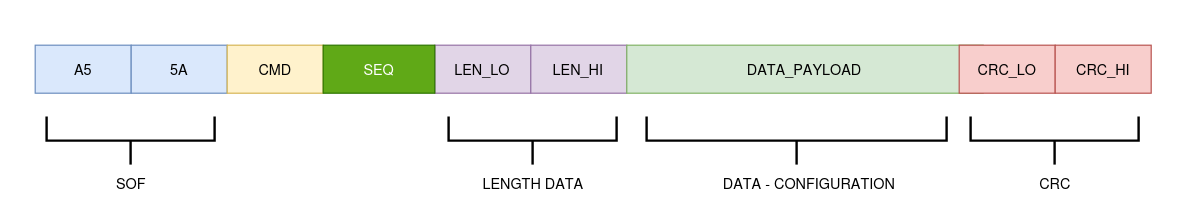
\includegraphics[width=0.96\textwidth]{ch05_giao_thuc_uart/frame.png}
  \caption{Cấu trúc khung gói UART.}\label{fig:khungoi}
\end{figure}

Khung gói gồm $8$~byte bao gói cố định và phần tải dữ liệu:
\begin{itemize}
  \item \textbf{\texttt{SOF} (\texttt{0xA5}, \texttt{0x5A}):} $2$~byte đồng bộ đầu khung; phần thân gói được đếm theo độ dài \texttt{LEN} nên các byte trùng giá trị \texttt{SOF} trong vùng tải vẫn truyền bình thường.
  \item \textbf{\texttt{CMD} và \texttt{SEQ} ($1$~byte mỗi trường):} \texttt{CMD} mang mã lệnh ở chiều xuống (\texttt{0x08}--\texttt{0x15}) hoặc loại trả lời ở chiều lên (\texttt{0x80} \texttt{ACK}, \texttt{0x81} \texttt{NACK}, \texttt{0x82} \texttt{RESULT}); \texttt{SEQ} là số thứ tự gói do host cấp và được FPGA sao chép lại vào khung trả lời.
  \item \textbf{\texttt{LENGTH DATA} (\texttt{LEN\_LO}, \texttt{LEN\_HI}):} độ dài tải kiểu \texttt{u16} ($0\le\texttt{LEN}\le\texttt{MAX\_PAYLOAD}$).
  \item \textbf{\texttt{DATA\_PAYLOAD} (\texttt{LEN}~byte):} chứa địa chỉ, tham số cấu hình hoặc dữ liệu truyền nhận; bỏ qua khi $\texttt{LEN}=0$.
  \item \textbf{\texttt{CRC} (\texttt{CRC\_LO}, \texttt{CRC\_HI}):} mã kiểm tra dư thừa vòng (Cyclic Redundancy Check, CRC) $16$~bit tính từ byte \texttt{CMD} đến hết \texttt{DATA\_PAYLOAD}.
\end{itemize}

Cả chiều thu và chiều phát đều dùng chuẩn CRC-16/CCITT-FALSE (đa thức \texttt{0x1021}, giá trị khởi tạo \texttt{0xFFFF}) thông qua mạch tổ hợp \texttt{crc16\_ccitt\_next} (\texttt{comm/\allowbreak crc/\allowbreak crc16\_ccitt\_next.v}) cập nhật một byte mỗi chu kỳ xung nhịp.
Trong \texttt{packet\_rx} (\texttt{comm/\allowbreak protocol/\allowbreak packet\_rx.v}), các byte tải được ghi vào thanh ghi đệm tạm và chỉ phát xung \texttt{packet\_valid} sau khi kiểm khớp hai byte CRC cuối gói; nếu vượt \texttt{MAX\_PAYLOAD} hoặc sai CRC, mạch phát xung \texttt{packet\_error} để bộ điều khiển trả tín hiệu từ chối (Negative Acknowledge, NACK) mã~$1$ mà không ghi vào bộ nhớ truy cập ngẫu nhiên tĩnh (Static Random-Access Memory, SRAM).
Khi đang nhận dở một khung mà không có byte mới trong khoảng \texttt{RX\_TIMEOUT\_CLKS} ($\texttt{CLK\_FREQ}/10$) hoặc có xung \texttt{frame\_error}, \texttt{packet\_rx} tự đưa trạng thái về chờ \texttt{0xA5}.

Tham số \texttt{MAX\_PAYLOAD} của thiết kế là $128$~byte (trả trọn $64$~giá trị $16$~bit của bộ nhớ trung bình toàn cục --- Global Average Pooling, GAP --- trong một khung).
Đối với các lệnh ghi mảng có $2$~byte địa chỉ ở đầu tải, mỗi gói mang tối đa $126$~byte dữ liệu và các mảng lớn hơn được host tự động tách thành nhiều khung nối tiếp.
